\chapter{相关工作}
本文实验的系统,与信息抽取、本体学习等领域有较强的相关性,同时用到了自然语言处理、机器学习的一些模型和方法。下面对本文主要的相关工作作简单的介绍。
\section{信息抽取}

信息抽取(Information Extraction)是文本挖掘和信息检索中的一项重要任务,它的目标是从非结构化或半结构化的信息中发现结构化的特定信息,其中命名实体抽取,如人名、组织、地点,是最基础的任务,更复杂的抽取任务,如事件、关系抽取,依赖于精准的命名实体抽取。

信息抽取中早期的工作通常基于规则\cite{ciravegna2001adaptive}。首先,手工设计或者自动生成一系列规则,文本中的每个符号都被表示为特征的集合。一条规则包含一个正则表达式和动作。例如,一个识别人名的规则如下:
\begin{center}
	(第一个词:``Mr.'',第二个词:首字母大写) $\rightarrow$ 人名
\end{center}
将文本和规则匹配,如果匹配成功,则执行对应的动作。如果有多条规则,需要定义规则执行的顺序,例如顺序执行.

在特定的任务上基于规则的方法可以达到很好的性能,但是设计良好的抽取规则依赖于领域专家大量的工作,费时费力,并且针对一个目标的工作无法应用到其他目标中。因此,研究者之后将统计机器学习应用到信息抽取中,将信息抽取分解为不同的子问题,这些子问题可以转化为分类问题,可以使用支持向量机、最大熵模型等解决。信息抽取有时需要辨别文本的不同部分的语义角色,因此序列标注的方法被广泛应用。为了把实体抽取问题映射到序列标注问题,将句子中的每个词作为观察值,用BIO表示法标记文本块的边界。对每个实体类型T,类标B-T表示一个类型为T的实体名称开始,I-T表示位于T类型实体名称内部,O表示在任何一个名称外部,序列标注问题在于给出一个词序列,求出统计意义下最可能的标注序列。

\begin{problem}[序列标注]
已知观察值${\bf{x}} = ({x_1},{x_2}, \ldots {x_n})$,求最优序列标注${\bf{y^*}} = ({y_1},{y_2}, \ldots {y_n})$, 使得${{\bf{y}}^*} = \arg {\max _{\bf{y}}}P({\bf{y}}|{\bf{x}})$.
\end{problem}
在隐马尔科夫模型(HMM)中,对序列的生成过程做了两个假设。1,马尔科夫假设,即每个类标$y_i$仅由前一个类标$y_{i-1}$生成;2,输出独立性假设,输出观察值之间严格独立。状态的转移概率可以在语料中进行频度估计,如
\[
p(y_i=c|y_{i-1} = c, x_{i-1}=w) = \frac{n(c_1, c_2, w)}{n(c_2, w)}
\]
为了避免数据稀疏性的问题,可以加入必要的光滑。

HMM是一个生成模型,但它的两个假设有时并不合理。当数据较充足时,直接对$P(y|x)$进行建模的判别模型可能有更低的预测误差。McCallum等人将最大熵马尔科夫模型(MEMM)应用于信息抽取\cite{mccallum2000maximum},修正了观察值之间严格独立的假设。在MEMM中,同样有马尔科夫假设,类标$y_i$依赖于附近的观察值$x_{i - l}^{i + l} = ({x_{i - l}},{x_{i - l + 1}}, \ldots ,{x_{i + l}})$和之前若干个类标$y_{i - k}^{i - 1} = ({y_{i - k}},{y_{i - k + 1}}, \ldots ,{y_{i - 1}})$:

\[p({\bf{y}}|{\bf{x}}) = \prod\limits_i {p({y_i}|y_{i - k}^{i - 1},x_{i - l}^{i + l})} \]

其中
\begin{equation}
{p({y_i}|y_{i - k}^{i - 1},x_{i - l}^{i + l})} = \frac{{\exp \left( {\sum\limits_j {{\lambda _j}{f_j}({y_i}} ,y_{i - k}^{i - 1},x_{i - l}^{i{\rm{ + }}l})} \right)}}{{\sum\limits_{y'} {\exp \left( {\sum\limits_j {{\lambda _j}{f_j}(y'} ,y_{i - k}^{i - 1},x_{i - l}^{i{\rm{ + }}l})} \right)} }} 
\label{eqn:memm}
\end{equation}
$f()$是定义在类标和观察值上的特征函数。

MEMM虽然不需要输出独立性假设,但由于MEMM只在局部做归一化\ref{eqn:memm},状态概率分布不平衡,存在标注偏置问题(label bias problem)。条件随机场(CRF)\cite{lafferty2001conditional}解决了这一问题。CRF和MEMM的区别有:1,$y_i$不仅和$y_{j<i}$有关,而且和$y_{j>i}$有关;2,CRF是一个无向图模型,而MEMM是有向图模型;3,CRF做全局归一化,而不是局部归一。在一阶线性CRF中,
\[ p({\bf{y}}|{\bf{x}}) = \frac{1}{Z}\exp (\sum\limits_i {\sum\limits_j {{\lambda _j}{f_j}({y_i},{y_{i - 1}},{\bf{x}},i)} } \]
$Z$为归一化常数,	
\[{\rm{Z = }}\sum\limits_{{\bf{y'}}} {\exp (\sum\limits_i {\sum\limits_j {{\lambda _j}{f_j}({y_i},{y_{i - 1}},{\bf{x}},i)} } }) \]

CRF是当前使用最广泛的信息抽取模型,并且在此基础上有许多工作对其进行发展。例如,为了克服CRF难以引入长程特征的问题,Sarawagi\cite{sarawagi2004semi}提出了Semi-Markov CRF,它可以在较低的计算消耗下,达到和高阶CRF相似的预测能力。

\begin{figure}[h]
\centering
\begin{subfigure}{0.3\textwidth}
\includegraphics[width=\textwidth]{HMM.png}
\caption{HMM}
\end{subfigure}

\begin{subfigure}{0.3\textwidth}
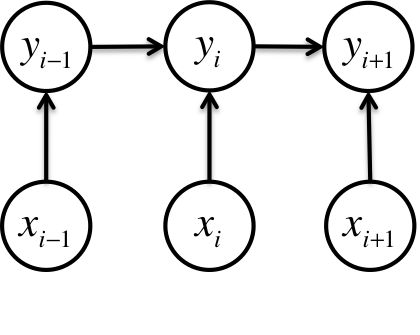
\includegraphics[width=\textwidth]{MEMM.png}
\caption{MEMM}
\end{subfigure}

\begin{subfigure}{0.3\textwidth}
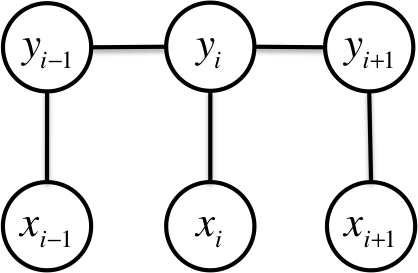
\includegraphics[width=\textwidth]{CRF.png}
\caption{CRF}
\end{subfigure}

\caption{序列标注模型}
\label{fig:seq_label_model}
\end{figure}

\section{本体学习和概念层次构建}
本体学习(Ontology Learning)是从自然语言文本中自动抽取概念及其关系的过程,它与信息抽取有着密切的联系,但是本文关注其中的一个重要子任务,将抽取出的概念组织为层次化的分类系统(hierarchy induction)。话题层次、概念层次是对数据不同粒度上的组织,有许多重要应用,如基于本体的个性化Web搜索和浏览\cite{gauch2003ontology}。对概念进行层次化的建模,可以使用基于统计或基于词法、语法模式的方法。当前大多数的工作集中于挖掘上下位关系,即is-a关系。Rion Snow\cite{snow2004learning}提出了一个上下位关系的学习模型。对于给定的两个词$c_i,c_j$,他首先找到语料中包含这两个词的所有句子,并进行句法解析得到依赖树,随后基于语法特征训练分类器,预测两个词之间是否存在上下位关系。Roberto Navigli\cite{navigli2011graph}提出了一种新颖的基于图的方法。他首先将不同的概念组织成有向图,这张图可能是稠密、带环甚至是不连通的,图的边表示概念的关系,可以用之前的方法生成。随后从最一般的概念开始,寻找最优分支,修剪有噪声的边,得到分类层次。

这些传统的层次构建方法均需要一个领域相关的语料。但不足在于,
\begin{enumerate}
\item 与目标领域高度相关的语料常常是难以获得的,例如,``计算机科学''相关的语料库很容易获得,但仅和``模式识别''相关的语料就不容易了;并且我们常常关注崭新的、不断变化的领域,相关语料更难以获得。
\item 为了构建概念之间的关系,常常要从中找出一些语言模式。而高质量的模式是稀疏的,尤其是语料不足时。
\end{enumerate}
Xueqing Liu等人\cite{liu2012automatic}提出了一种基于关键词集合的层次构建方法。对于每个关键词,从知识库中获取相关概念,并从搜索引擎中获取上下文信息,然后进行多分支的层次聚类方法Bayesian Rose Tree进行聚类,得到新的类别层次。BRT的构建过程中,最初所有数据点被作为独立的树$T_i=\{\bf{x}_i\}$。使用贪心策略,每次迭代选取两棵树$T_i$和$T_j$,将其合并为一棵新树$T_m$。与二叉的层次聚类不同,BRT有三种可能的操作:
\begin{itemize}
\item 合并(Join)。$T_m=\{T_i, T_j\}$, 即$T_i, T_j$作为$T_m$的子树。
\item 吸收(Absord)。$T_m  = \{children(T_i) \cup T_j\}$, $T_m$有$|T_i|+1$个子结点。
\item 坍缩(Collapse)。$T_m = \{children(T_i)\cup children(T_j)\}$,$T_m$有$|T_i|+|T_j|$个子节点。
\end{itemize}
选取$T_i, T_j$和合适的操作,使得最大化
\[
\frac{p(D_m|T_m)}{p(D_i|T_i)p(D_j|T_j)}
\]
其中$p(D_m|T_m)$是$T_m$下所有叶节点数据点,$D_m=\{ D_i\cup D_j\}$。$p(D_m|T_m)$递归定义为
\[
p(D_m|T_m) = \pi_{T_m}f(D_m)+(1-\pi_{T_m}) \prod \limits_{{T_i} \in Children({T_m})} {p({D_i}|{T_i})} 
\]

Chi Wang\cite{wang2013phrase}提出了基于共现的对短语进行层次话题挖掘的框架。对本文的工作有很大启发。

\section{活动挖掘}
现阶段,对用户活动进行挖掘的工作十分有限。可以找到的工作有Nguyen Minh The以及Keun Chan Park\cite{park2010detecting}。Nguyen\cite{the2010automatic}\cite{kawamura2010human}提出了使用了自监督条件随机场(self-supervised CRF)从博客中挖掘用户活动的系统,目标在于抽取活动的基本属性:参与者(actor), 动作(action), 对象(object), 时间(time),地点(location)。Nguyen工作的特点在于,借助了语法正确,易于解析的维基百科中人物类目的语料,通过语法模板进行自动标注,作为训练数据,训练CRF抽取模型。这个系统包含两个模块
\begin{enumerate}
\item 自监督学习模块
\item 活动抽取模块
\end{enumerate}
如图\ref{fig:nguyen_frameword}所示
\begin{figure}[!h]
\centering
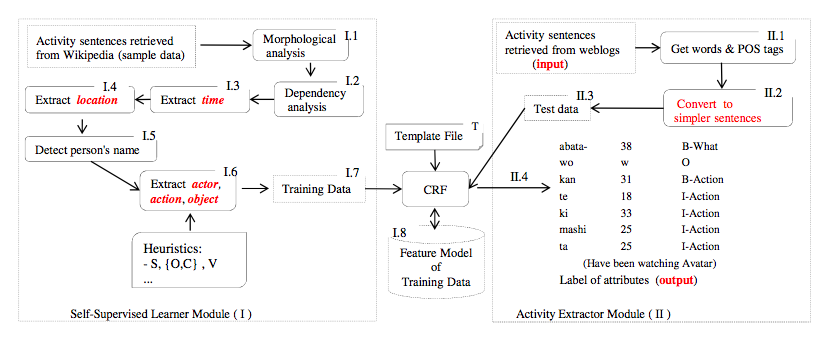
\includegraphics[width=\textwidth]{arch_Nguyen}
\caption{Nguyen的活动抽取框架}
\label{fig:nguyen_frameword}
\end{figure}

主要步骤如下
\begin{itemize}
\item 对维基百科的语料进行分词、词性标注和句法解析,得到词性标签和短语依赖关系,如动词短语(VP), 名词短语(NP),命名实体。
\item 使用Google Map API进行地点标注。
\item 手动设计一系列的语法模板,如``S, \{O,C\}, V'',``\{O, C\}, V, S'',其中S表示主语,O表示对象,V表示动作,C表示补语。根据这些语法模板,可以获得包含活动的句子,并标注活动的参与者,动作和对象。
\item 使用以上步骤得到的语料,训练CRF,获得一系列特征函数。
\item 在活动抽取模块中,使用训练的到的CRF模型解析,获得抽取结果。
\end{itemize}

但是Nguyen的工作关注的是博客(Weblog)内容的抽取,博客和微博的形式有比较大的区别,一方面,博客长度没有限制,一般是对一个活动的完整叙述,信息完整;另一方面,博客的写作也更加严谨,语法结构比较正式。此外,这个系统仅仅关注信息的抽取,并没有对活动进行更进一步的挖掘。因此,他的工作难以直接应用于本文的工作。本文从短语着手,并充分利用了微博的元信息,克服了这些问题。

\section{情感分析}
本文的工作中,需要对用户参与一项活动的情感状态进行分析。情感分析(Sentiment Analysis)和观点挖掘(Opinion Mining)是信息检索的一个重要研究领域,在过去十多年中,学界已有许多工作,也有许多商业公司提供观点挖掘的服务。
一个完整的观点挖掘任务的目标在于,给定带有观点的文档集$D$,发现其中包含的所有观点,每个观点可用五元组$(e_i, a_{ij}, oo_{ijkl},h_k, t_l)$表示,其中
\begin{itemize}
\item $e_i$:观点相关的实体名称
\item $a_{ij}$:$e_i$的一个方面(aspect)
\item $oo_{ijkl}$:观点的情感极性,如正面,负面,中性,或者一系列情感强度
\item $h_k$:观点的持有者
\item $t_l$:观点的发表时间
\end{itemize}

情感分析可以在不同的粒度进行。文档级的情感分类假定文档$d$仅对一个实体$e$发表观点,且观点仅来自一个用户$h$,仅判断其情感极性,它是情感分析工作的基础。
它是一个分类问题,现有的有监督学习方法均可应用在情感分类中。Bo Pang等人\cite{pang2002thumbs}使用unigram作为特征对文档进行二分类,发现朴素贝叶斯和SVM均有很好的表现。随后的工作\cite{pang2008opinion}利用了更多的特征,如
\begin{itemize}
\item 词组及词频
\item 词性标签。形容词是观点的重要标志,因此作为单独的特征
\item 观点词。收集人们经常使用的表达观点的词,如动词``喜欢'',``讨厌'',形容词``不错'',``差''作为特征,对于提高精度有很大帮助。
\item 否定词。句子中的否定词可能会改变情感极性,因此也作为特征。
\end{itemize}

非监督方法也可应用于情感分类。Turney等人\cite{turney2002thumbs}提出了一个非监督的框架。首先抽取出包含形容词的短语集合$\{p_i\}$,对每个短语$p_i$, 计算与已知情感极性的常见词的PMI,作为情感倾向
\[
SO(p_i) = PMI(p_i, \text{``excellent''}) - PMI(p_i, \text{``poor''})
\]
最后,对于给定的文档,计算所有形容词短语的平均情感倾向得分$SO$,若为正,则归类为正面,否则为负面。

尽管从文档级别对情感进行分类大多数情况下是有用的,但在很多应用中,它没有没有提供足够的细节。一个关于特定实体$e$的正面文档并不意味着作者对$e$的所有方面都有正面的评价。因此,需要进行更细粒度的基于方面的情感分析(Aspect-based Sentiment Analysis),它可以分为两个子任务:
\begin{itemize}
\item 方面抽取
\item 情感分类
\end{itemize}
两个子任务可以依次进行,分别利用信息抽取相关工具和文档/句级情感分类工具完成相关工作。Topic Modeling的方法也被尝试用于非监督的观点抽取,许多工作在LDA的基础上进行扩展,增加表示情感和方面的隐层,同时对Aspect和Opinion词进行建模,Wayne Zhao等人提出的MaxEnt-LDA是其中比较有代表性的工作\cite{zhao2010jointly}。如图\ref{fig:maxent_lda}, 文档中的每个词$w_{d,s,n}$由多个Mixture产生:背景词\ $\Phi^B$, 全局Aspect\ $\Phi^{A,g}$, 全局Opinion\ $\Phi^{O,g}$, 某个特定Aspect\ $A_t$, 某个特定Opinion\ $O_t$,并由Bernoulli变量$y_{d,s,n}$和$u_{d,s,n}$抽样得到由哪一个Mixture产生。他们的工作借助了语法特征,帮助将Aspect词和Opinion词区分开,解决了此前工作的	问题\cite{titov2008modeling}。

本文的工作中,由于微博本身的特性,为了简化问题,主要进行文档级的情感分析。

\begin{figure}[!h]
\centering
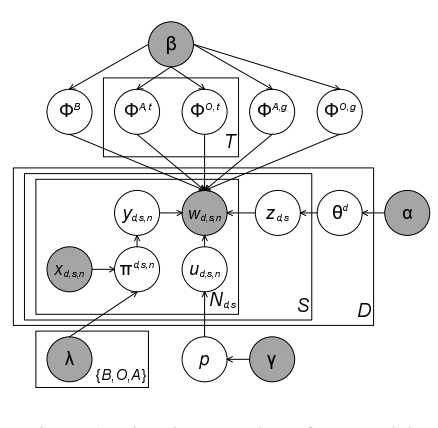
\includegraphics[width=0.6\textwidth]{MaxEntLDA.png}
\caption{MaxEnt-LDA}
\label{fig:maxent_lda}
\end{figure}

\section{现有知识库系统概况}
知识库是对人类知识的结构化表示,它在搜索、智能系统中有着日益重要的应用,Google,Microsoft以及国内百度、搜狗等互联网企业均有自己的知识图谱计划。本文的工作目标就在于构建一个关于人类日常活动的知识库。表\ref{table:knowledge_base}对研究工作中常见的知识库的概况进行了总结。

\begin{table}[!h]
\begin{tabular}[0.7\textwidth]{|l|p{2cm}|l|l|p{4cm}|}

\hline
名称 		& 开发者 & 概念数量 & isA关系数量 & 概述 \\
\hline
SenticNet	& 南洋理工大学、新加坡国立大学 & 14,244 & NA & 借助图挖掘和数据降维,提供了概念级的情感分析资源。 \\
\hline
Freebase	& 社区	& 1450	& 24,483,434 & 常用的开放知识库系统。对不同领域的知名人物、地点、事物根据Topic组织归类,提供搜索和API查询 \\
\hline
WordNet\cite{miller1995wordnet} & 普林斯顿大学 & 25,229 & 283,070 & 英语词汇的知识库,根据同义语将英语词汇进行组织,并且提供词汇之间的多种语义关系。 \\
\hline
WikiTaxonomy\cite{ponzetto2007deriving}	& HITS & 127,325 & 105,418 & 基于维基百科(Wikipedia)的语料, 将类别按照is-A关系构建为一个大规模分类系统 \\
\hline
Probase & Microsoft & 2,653,872 & 20,757,545 & 借助数十亿的网页和多年的搜索记录,构建了比传统知识库庞大许多的概念。并且对不确定性进行建模,以此为基础实现概率推理的功能。 \\
\hline
\end{tabular}
\caption{现有知识库概况}
\label{table:knowledge_base}
\end{table}

从表\ref{table:knowledge_base}中可以看到,现有的知识库种类繁多,其中Probase在系统规模和功能上达到了很高的水准,但现有的知识库系统主要关注客观实体如人物、地点、物体及其关系建模,没有一个针对人类日常活动的知识库系统。希望我的工作能在这方面对现有的知识库的一个补充。


